%%% Local Variables:
%%% mode: latex
%%% TeX-master: t
%%% End:

\documentclass[12pt,a4paper,titlepage]{article}
\usepackage[style=numeric,backend=bibtex,firstinits=true,maxbibnames=99]{biblatex}
\usepackage{graphicx}
\usepackage{enumitem}
\usepackage{amssymb}
\usepackage[utf8]{inputenc}
\usepackage{rotating}
\usepackage{float}
\usepackage{pgfplots}
\usepackage{subcaption}

% \pgfplotsset{compat=1.10}

\usepgfplotslibrary{fillbetween}

\newcommand{\co}[1]{\texttt{#1}}
% TODO: choose this (small caps, monospace, sans serif)

\graphicspath{ {images/} }
\bibliography{report.bib}


\begin{document}

\begin{titlepage}

\newcommand{\HRule}{\rule{\linewidth}{0.5mm}} % Defines a new command for the horizontal lines, change thickness here

\center % Center everything on the page
 
\textsc{\LARGE University of Oxford}\\[1.5cm] % Name of your university/college
\textsc{\LARGE Honour School of Computer~Science \\[0.2cm] and Philosophy}\\[0.5cm] % Major heading such as course name

\HRule \\[0.4cm]
\textbf{\LARGE Approximating Walrasian Equilibria} \\[0.3cm]
\textbf{\LARGE with Decentralized Bilateral Trade}\\[0.1cm]
\HRule \\[2cm]
 
\begin{minipage}{0.45\textwidth}
\begin{flushleft} \Large
\emph{Author:}\\
Victor Porras % Your name
\end{flushleft}
\end{minipage}
~
\begin{minipage}{0.45\textwidth}
\begin{flushright} \Large
\emph{Supervisor:} \\
Professor Paul Goldberg % Supervisor's Name
\end{flushright}
\end{minipage}\\[2cm]

{\Large {May 2017}}\\[2cm]

% \includegraphics[scale=0.2]{images/logo.png}
 
%----------------------------------------------------------------------------------------

\vfill % Fill the rest of the page with whitespace

\end{titlepage}

\begin{abstract}
  We study the Walrasian equilibria of markets with $n$ traders and 2 goods.
  We simulate the convergence of such a market through decentralized randomized bilateral trade.
  Traders learn constraints on the prices of the goods to minimize loss of wealth.
  To avoid divergence while searching for constraints, we introduce the technique of backtracking.
  We show that our algorithm is stable across different randomizations.
\end{abstract}

\tableofcontents
\newpage

\section{Introduction}
Billions of people around the world trade goods and services on markets every day.
With few exceptions, prices are stable enough that people can plan for the future, but dynamic enough to balance supply and demand.
These prices make it possible for producers to make the right amount of commodities for consumers thousands of kilometres away, and for consumers to buy them as cheaply as possible.
In economics, we say that prices can form an equilibrium when they stabilize.

The equilibrium conditions of markets have been widely studied in economics for hundreds of years.
Equilibrium theory is important for understanding how markets arrive at prices, especially after shocks. 
It is also used to develop and test both macro and microeconomic models. 
Economic models are ultimately useful for making economic forecasts.
We want to make the best predictions possible as well as understand why certain predictions fail.
For example, we want to know why prices can settle even in decentralized markets, where buyers and sellers transact directly, without a central intermediary.
On the other hand, financial markets have turbulent prices despite rapid information sharing and price discovery.

A Walrasian equilibrium (WE) is a useful formalization of an equilibrium in a competitive market.
Essentially, it is a set of prices at which the supply of every good equals its demand.
We give a rigorous definition in Section \ref{background}.
There are many fast algorithms for calculating the WE of a market when there is access to a central information source.
These are useful for modelling official markets with a central trading venue and easily accessible price data, like a stock exchange or an art auction.
Decentralized markets have been less studied, but they are also a crucial part of trade.
For example, while stocks are usually traded on public exchanges, bonds are still mostly traded over the phone, in private.
Other goods are traded even more informally, some via online markets like Craigslist and Gumtree.
Understanding how prices evolve in these markets is crucial to understanding the modern economy.

The purpose of this project is to learn how decentralized algorithms for calculating the WE, like that suggested by Crockett, Spear, and Sunder \cite{crockett}, perform in practice.
We investigate finding an approximate WE using bilateral trade.
In a given trading day, random pairs of traders make the largest trade possible until nobody can make any more trades. 
Following each day, the traders update constraints on the prices they are willing to accept.
After many days of tightening constraints, the market should converge to a stable set of prices and allocations, the approximate WE.
We implemented this algorithm in Python and experimented with different techniques of updating the constraints.
% TODO: Why? What is the point of implementing this? To get some kinds of insight? What are they?

The naive implementation of this algorithm often failed to converge, and would instead diverge catastrophically, as the traders become over-constrained.
That made it unsuitable for finding the WE of a market.
To solve the problem of divergence, we developed a technique of backtracking to previous constraints with some probability when utility fell below a threshold.
This made it possible to reliably simulate a market and obtain useful results.

We show that with backtracking, this algorithm finds approximate Walrasian equilibria consistently, and does not diverge.
We also show that the randomized algorithm gives the same results for a given endowment across multiple runs with different random numbers.
Lastly, we extend the algorithm to work without access to the gradient of the traders' utility functions.

Section~\ref{background} is an explanation of the economic aspects of the project and its relation to previous work.
In Section~\ref{desimp}, we discuss the model we use and the choices we made when implementing it.
Section~\ref{results} contains the results we obtained from our simulations.
We analyse the success of the project and compare it to other methods in Section~\ref{conclusion}. 

\section{Background}\label{background}

This project focuses on simulating a world with multiple traders that exchange two divisible goods amongst themselves.
An assignment of goods to traders is called an \textit{allocation}.
Each trader in our world will receive an initial \textit{endowment} allocation of goods, which they can trade with the others.
Thus, the allocation will change throughout a day of trading.

The \textit{marginal rate of substitution} (MRS) between the two goods will be used throughout to represent price.
It applies to both potential and actual trades.
We always express the MRS and gradient (defined below) as units of good 2 per unit good 1.
For instance, a trade of 4 units of good 1 for 1 unit of good 2 has an MRS of 0.25.

The \textit{direction} of a trade is either ``Buy'' or ``Sell'', from the perspective of a given trader.
Direction is also expressed in terms of good 1, so a ``Buy'' means the trader is gaining good 1 by giving up good 2.
The direction is antisymmetric: a ``Buy'' for one trader is a ``Sell'' for their trading partner.
% TODO: check with Toby: antisymmetric the right word here?

Utility functions capture the preferences of the actors in an economic model.
Utility is often associated with the pleasure or satisfaction that an actor gets from a situation.
A rational actor, by definition, always prefers an outcome with higher utility to one with lower utility. 
In general, a utility function is a function from states of the world to utilities.

Consider a market with $m$ traders and $n$ goods, where each trader $i$ begins with an endowment $\mathbf{w}_i \in \mathbb{R}^n_+ $ of some goods.
Let $u_i : \mathbb{R}^n_+ \rightarrow \mathbb{R}$ be the utility function for trader $i$.
A Walrasian equilibrium (WE) is a set of prices $\mathbf{p} \in \mathbb{R}^n_+$ and allocations of goods $\mathbf{x}_i \in \mathbb{R}^n_+$ which satisfies the following conditions:
\begin{equation}\label{eq:goods}
  \sum_i \mathbf{x}_i = \sum_i \mathbf{w}_i 
\end{equation}
\begin{equation}\label{eq:prefs}
  u_i(\mathbf{x'}) \leq u_i(\mathbf{x}_i) \quad
  \forall{i} \; \forall{\{\mathbf{x'} \in \mathbb{R}^n_+ \mid \mathbf{p} \cdot \mathbf{x'} \leq \mathbf{p} \cdot \mathbf{w}_i}\}
\end{equation}
\begin{equation}\label{eq:wealth}
  \mathbf{p} \cdot \mathbf{x}_i = \mathbf{p} \cdot \mathbf{w}_i \quad \forall{i} 
\end{equation}

% TODO: check these maths with Toby

An approximate WE relaxes one of these conditions.

Condition \ref{eq:goods} requires that the amount of each good is constant.
This should be true no matter what trading occurs.

Condition \ref{eq:prefs} means that the allocations are rational for the traders.
They would not prefer any other allocation of the same or less value.
If the first and second conditions hold, the allocation is Pareto-optimal.
% TODO: reference/explain Pareto?

Condition \ref{eq:wealth} requires that the traders do not gain or lose wealth during the trading.
Intuitively, this means the traders can ``afford'' their final allocations.
This is the condition we will relax.

For this model, a utility function is $\mathbb{R}^2_+ \rightarrow \mathbb{R}$ from the allocations of each good.
We use the Cobb-Douglas utility function:
\[
  u(x, y) = x^p y^{(1-p)}
\]
where x and y are the quantities of the goods.
The parameter p is adjusted to give traders different preferences.

% TODO: rephrase this for clarity, explain contour, diagram?
Because this function is differentiable, we can calculate the gradient.
This makes it possible to calculate the slope of the line tangent to the indifference contour, which is
\[
  \frac{(1-p)y}{px}
\]
This slope is a bound on the MRS that a trader can accept for the trade to increase their utility.

Closely related to utility is the concept of wealth.
Given allocation $\mathbf{x}$ and MRS $p$, wealth is $ px_1 + x_2 $.
Utility is a subjective measure based on the trader's preferences, while wealth is objective and based on the market.
While it is impossible for a trader to lose utility during a day, they can lose wealth.
This can happen when one trader has a disproportionately high amount of a good that a market values.
They can sell it too cheaply at first, when they could have demanded a higher price.
When this occurs, the trader who loses wealth is called a subsidizer.
This terminology was introduced by Crockett et al. \cite{crockett}.

We will refer to the random number generator later in this report.
As in most applications, we actually use a \textit{pseudo-random} number generator.
This is a function which takes a \textit{seed} and produces a sequence of seemingly random numbers.
The crucial part is that the same seed will always produce the same sequence.
For other programs, the current time is often used as a seed so the sequence is not repeated.
However for our purposes, we will use specific seeds to get reproducible results and still reap the benefits of a randomized algorithm.

There is a long history of trial-and-error techniques in this field.
Walras' original idea for finding equilibrium is called \textit{tâtonnement}, which literally means trial-and-error in French.
His approach was to have a centralized auctioneer pick a price, calculate the aggregate supply and demand, then adjust the price accordingly.
This seems very plausible, and it does work in practice for some special cases.

However, Scarf showed that there were initial allocations which could be chosen so as to be unstable under this procedure \cite{scarf}.
Later research demonstrated that a modified tâtonnement procedure could be found, but only if the auctioneer has knowledge of all the traders' utility functions, including their gradients.
% TODO: Cite the later research. Give references.

Crockett et al. investigate using trading to solve the divisible goods case \cite{crockett}.
They pioneer the use of constraints learned by traders to reach a WE and prove convergence guarantees for the two-trader case.
Unfortunately, they also show that there are cases where bilateral trade cannot find an exact equilibrium in the multi-trader case.

In an unpublished note, Axtell and Goldberg \cite{goldberg} suggested finding the quantitative performance of the algorithm suggested by Crockett et al.
This would be useful because it could be used to simulate a real market without a central clearing house, unlike the algorithms which rely on an aggregate demand oracle.
We have used this as our starting point.


In this field, there are several different ways an equilibrium model can learn about the world. 
We use a utility oracle and a utility gradient oracle to access the preferences of traders for a given allocation.
At any one time, we only access the oracles for the two traders involved in a potential trade.
Significantly, the algorithm does not need to know anything about the whole system at once.
Another option is the aggregate demand oracle, which takes a vector of prices and gives the net supply and demand across the whole system; this is what tâtonnement uses to find an equilibrium.
This is realistic for some applications, like a store that only knows how much of a product it sells at each price.
Fleischer et al. give performance guarantees using an aggregate demand oracle to find the approximate WE \cite{fleischer}.
Their algorithm is a variation on tâtonnement.
% TODO: which variation? add more details
Leme and Wong also use an aggregate demand oracle to give a polynomial algorithm for the indivisible goods case \cite{leme}.

\section{Design and Implementation}\label{desimp}
We created a software framework to implement the algorithm above and test it with different parameters.
% TODO: Again, it would help if you explicitly stated your intent in implementing into this algorithm. 
We used Python to build it, because it allowed for rapid prototyping and flexible experimentation.
The program runs multiple trials using the same parameters, where each trial consists of many days of trading.
Here, we discuss the details of the algorithm as implemented, and the concepts that were important to the implementation.
In particular, we discuss the goal of convergence and the challenge of divergence.

\subsection{The Trading Day}

Each day of the simulation begins by giving each trader their initial endowment.
Then, pairs of traders are randomly selected to attempt a trade.
Each trader has access to their utility functions and the gradients of those functions for any allocation.
From the gradient and any constraints, we calculate two MRSs for each trader, one for each direction.
The direction of the potential trade (Trader 1 buying from Trader 2 or vice versa) is chosen based on the differences between their MRSs.
The trader with the higher MRS is the one who buys Good 1.
% TODO: diagram of trade.

In the standard model (see Section \ref{nograd} for the version without access to gradients), we calculate a joint MRS by taking the geometric mean of two MRSs.
This joint MRS is the exchange rate used for the potential.
We experimented with randomly picking an MRS between the two traders' MRSs, but this was slower and gave worse results.

Then, we calculate the size of the biggest possible trade that can occur at that MRS.
A trade can occur if, after reallocation, both traders would have higher utilities.
We test progressively larger sizes, doubling each time.
Because the gradient only applies to infinitesimally small sizes, when the MRSs are very similar, the minimum size might not be possible.
If the largest size is non-zero, the traders exchange the appropriate goods and the process repeats.
Figure \ref{fig:day} shows a day of trading with three traders.

As we go, we keep track of the most recent MRS each trader agreed to trade at.
We use this later on to assess the quality of the simulation.

The simulation of a day ends once traders can make no more mutually beneficial trades.
To check for this, we track the number of consecutive attempted trades that are rejected. 
For a simulation with $n$ traders, we wait for $n$ consecutive such empty trades.
There is a parameter that can increase or decrease this, but we found in practice that $n$ gives just as good results as $2n$ or $5n$, and is faster.
We do adjust that parameter when we get to the no-gradient case in Section \ref{nograd}.

\begin{figure}[H]
    \centering
    \includegraphics[width=\textwidth]{allocations_(seed_13).png}
    \caption{
      A single trading day for three traders.
      The green contours are lines of equal utility.
      Notice how the trades only increase utility.
      The red dots are the final positions of traders.
      The dotted lines are the bounds on the MRS.
      A trader will only trade above those lines.
      % TODO: explain this better
    }
    \label{fig:day}
\end{figure}

\begin{figure}[H]
  \centering
  \begin{subfigure}{.4\linewidth}\centering
    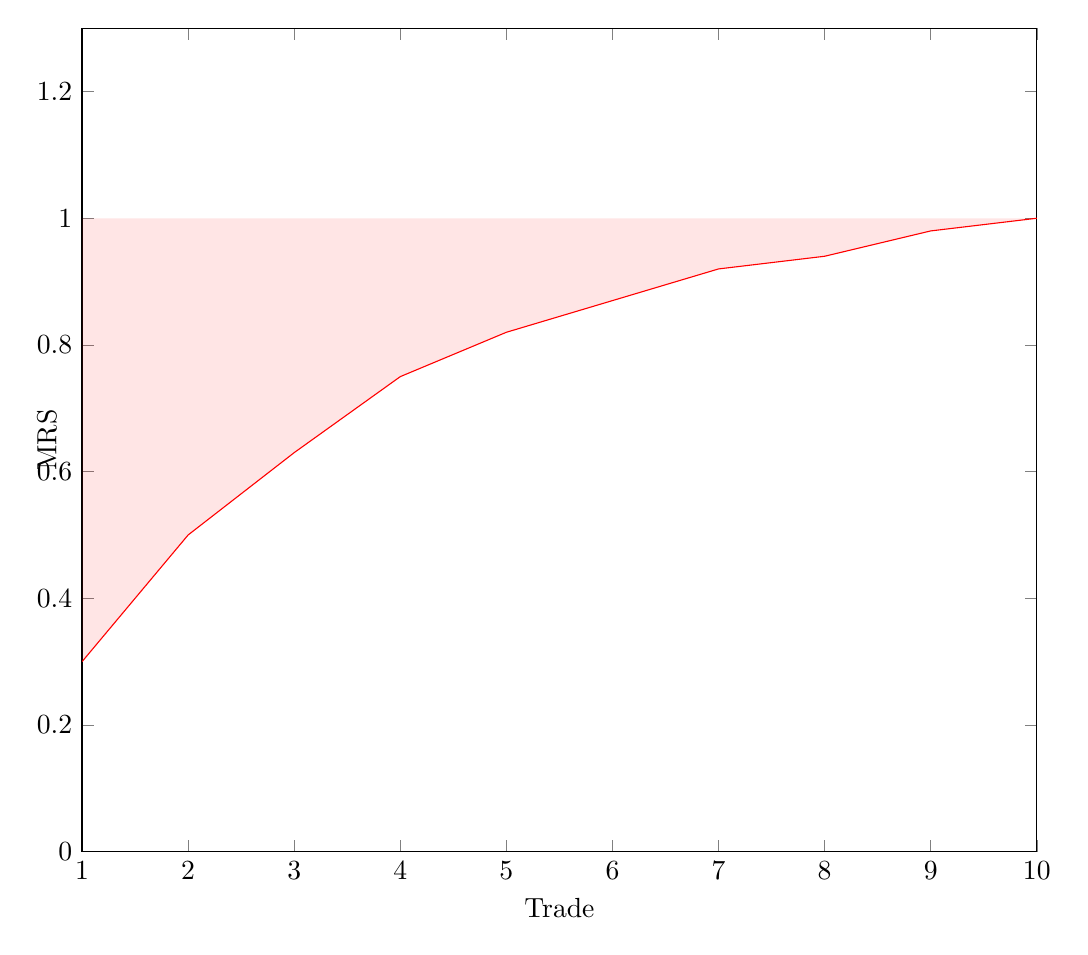
\begin{tikzpicture} 
      \begin{axis}[
        width=\linewidth,
        scale only axis,
        xlabel={Trade},
        ylabel={MRS},
        xmin=1, xmax=10,
        ymin=0, ymax=1.3,
        ylabel style={overlay, anchor=north,},
        ]
        \addplot[
          name path=f,
          color=red,
        ]
        coordinates {
          (1,0.3)(2,0.5)(3,0.63)(4,0.75)(5,0.82)(6,0.87)(7,0.92)(8,0.94)(9,0.98)(10,1.0)
        }; 
      
        \path[name path=axis] (axis cs:1,1.0) -- (axis cs:10,1.0);
      
        \addplot [
          thick,
          color=red,
          fill=red, 
          fill opacity=0.1
          ]
        fill between[
          of=f and axis,
          split,
        ];
      \end{axis}
    \end{tikzpicture}
    \caption{Without constraint}
  \end{subfigure}%
  \hfill
  \begin{subfigure}{.4\linewidth}\centering
    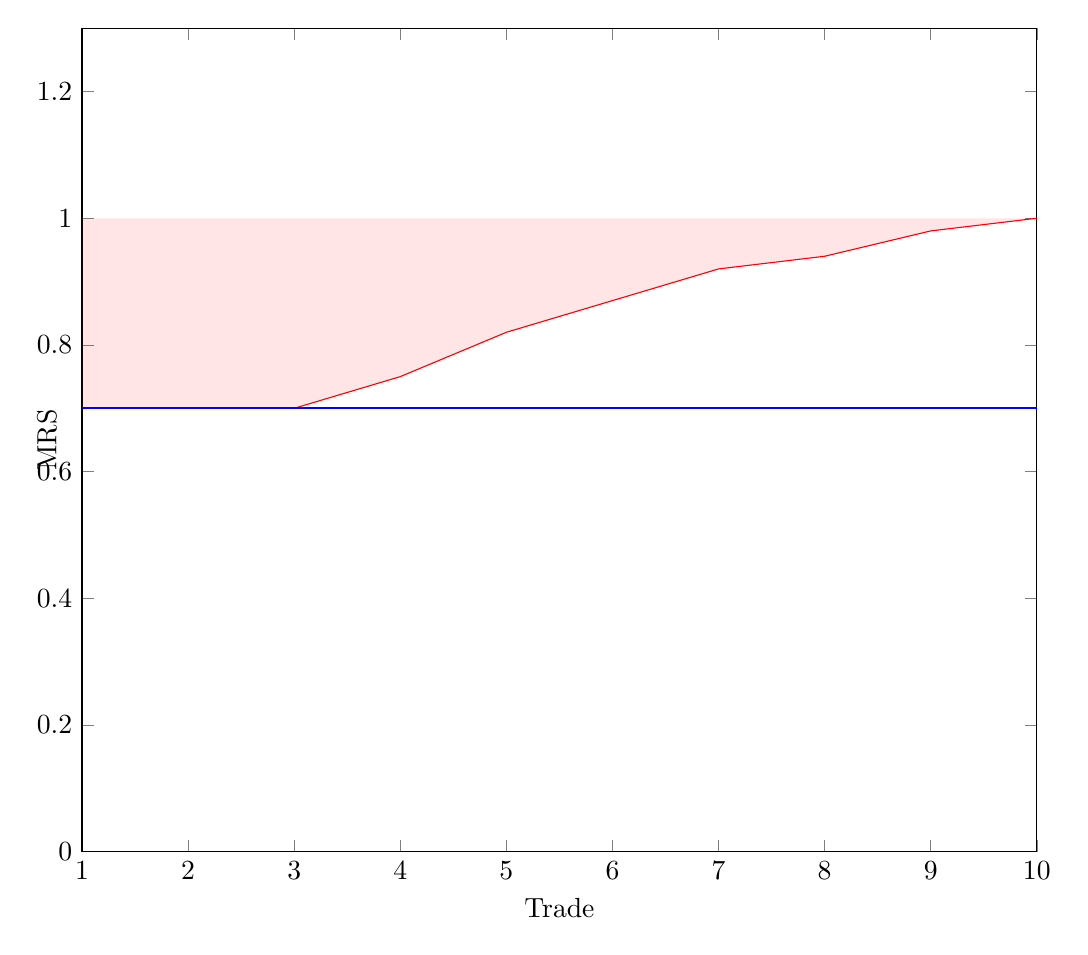
\begin{tikzpicture} 
      \begin{axis}[
        width=\linewidth,
        scale only axis,
        xlabel={Trade},
        ylabel={MRS},
        xmin=1, xmax=10,
        ymin=0, ymax=1.3,
        ylabel style={overlay, anchor=north,},
        ]
        \addplot[
          name path=f,
          color=red,
          ]
        coordinates {
          (1,0.7)(2,0.7)(3,0.7)(4,0.75)(5,0.82)(6,0.87)(7,0.92)(8,0.94)(9,0.98)(10,1.0)
        }; 
        
        \path[name path=axis] (axis cs:1,1.0) -- (axis cs:10,1.0);

        \draw[name path=constraint, color=blue, thick] (axis cs:1,0.7) -- (axis cs:10,0.7);
      
        \addplot [
          thick,
          color=red,
          fill=red, 
          fill opacity=0.1
          ]
        fill between[
          of=f and axis,
          split,
        ];
      \end{axis}
    \end{tikzpicture}  
    \caption{With selling constraint at 0.7}
  \end{subfigure}%
  
  \caption{
    This shows the MRSs that a subsidiser trades at over two days.
    The trader is selling, so they prefer a higher MRS.
    The shaded area is the wealth lost by not trading at the final price immediately.
    On the second day, the trader adds a selling constraint at 0.7, which means they lose less wealth.
    % TODO: more explanation
  }
  \label{fig:wealth}
\end{figure}

\subsection{Updating Constraints}
In order to get better outcomes from one day to the next, the traders must change their behaviour.
They achieve this by updating the constraints on the MRSs they will accept.

Each trader has two constraints: buying and selling.
The buying constraint is the highest MRS they will pay to buy good 1.
The selling constraint is the lowest MRS they will accept to sell good 1.

Using the definition of wealth from above, and the last MRS used globally, each trader calculates the wealth they gained or lost during the day.

Recall that no traders will accept trades that cause them to lose utility. 
Thus, they will have a non-negative utility gain, which we can calculate by subtracting the utility of the initial endowment from the utility of the final allocation after a day's worth of trades.

First, if the trader updated their constraint on the previous day, they evaluate its effectiveness.
They compare their wealth and utility gains from today to those from yesterday.
If the new constraint resulted in less utility or the same utility and less wealth, the constraint is reverted to its previous value.

If they did not update their constraint on the previous day, the trader considers tightening it.
\begin{itemize}
  \item If the trader gained wealth during the day, they are happy with the MRSs they are accepting, so they don't make any changes.
  \item If the trader lost wealth, they determine whether they were a net buyer or seller of good 1:
    \begin{itemize}
      \item If the trader was a net buyer, they decrease their buying constraint.
      \item If the trader was a net seller, they increase their selling constraint instead.
    \end{itemize}
\end{itemize}

See Figure \ref{fig:wealth} for an example of this procedure.
We will discuss the exact method of tightening in Section \ref{results}, when we compare different techniques.

\subsection{Statistics}
At the end of each day, we calculate five statistics about the day's trading: utility gain, wealth transfer, MRS deviation, constrainedness, and attempted trades.
These are used to evaluate the performance of the model.

The global utility gain, is the percentage increase in utility over the day for all the traders. 
Because it is a percentage, it can be compared across different starting allocations and numbers of traders.
It increases initially then settles as the traders learn constraints that help them maximize their utility gains.
It can decrease if the traders become over-constrained.

The wealth transfer is the sum of the absolute value of wealth gained or lost, divided by the total wealth at the beginning.
Like above, it is marked to the MRS of the final successful trade.
This should approach 0 as subsiders apply constraints to prevent themselves from losing wealth.

As mentioned above, each trader has a most recent MRS they personally traded at.
In the ideal case, these all converge to the same value over the day, because if two traders disagree about MRS they can make a mutually beneficial trade.
To evaluate how close a simulation comes to this ideal, we calculate the standard deviation of the most recent MRS for each trader.

We calculate constrainedness based on the constraints used by each trader in the past day.
There are initial buy and sell constraints that every trader begins with.
This is the percentage of the original range between constraints that traders accept on average.
We actually use the log range, because the initial constraints vary by orders of magnitude and the plain range would underweight the lower (sell) constraint.
For example, constrainedness of 100\% means that 100\% of MRSs (within those initial constraints) are accepted.
Constrainedness of 5\% means that only 5\% of MRSs are acceptable on average.
We expect this to decrease over multiple days, and converge to a low value.

Lastly, we record the average number of attempted trades per trader in the day.
We use this as our main method of comparing the running time of different models.
The elapsed clock time is also recorded, but this is less useful because it isn't comparable across machines.

We track these statistics over many days of trading, and use them to analyse the results.
They are displayed in charts like that in Figure \ref{fig:conv}.

\begin{figure}[H]
    \centering
    \includegraphics[width=\textwidth]{seed_5.png}
    \caption{
      Convergence for 100 traders.
      Notice how all the statistics stabilize, and MRS deviation is small.
    }
    \label{fig:conv}
\end{figure}

\subsection{Convergence}
When designing models, we want to maximize the probability that they converge to a stable set of MRSs that maximise utility.
In a fixed number of days, a trial is said to converge or not converge.
Intuitively, a trial converges when it stops getting better (or worse).
We define a \textit{convergence point} as the day at which the average wealth transfer stops changing, with the caveat that the trial does not meet the divergence criteria below.
The convergence point is significant because it reflects how long a model would take to simulate a market in practice.
We chose to run all trials for 500 days to capture all relevant behaviour, but the better models converge well before that.

More concretely, given a trial that has not diverged, the convergence point is the earliest day where the wealth transfer for all following days is within a threshold.
Experimentally, we have found that a threshold of 1\% seems to capture the examples that match the intuition above.

We defined convergence on wealth, not utility, because the utility was noisier and less like a monotonic function.
Also, since the goal of this project is to approximate an exact Walrasian equilibrium, we are trying to minimize wealth transfers.
It is possible that the ideal equilibrium actually has lower utility than the simulation, but the ideal wealth transferred is always zero, due to condition \ref{eq:wealth}.
In effect, our model converges to the exact value plus some $\epsilon$.
We want to know the value of $\epsilon$, as well as how long it takes to achieve it.

For each model, we record the percentage of trials that converged, as well as the average wealth transfer, utility gain, MRS deviation, and constrainedness at that point.
We also record those same statistics at the end of the trial, though they are typically very similar.
The advantage of recording them at the end is that they can be compared across convergent and divergent cases.

\begin{figure}[H]
    \centering
    \includegraphics[width=\textwidth]{seed_0.png}
    \caption{
      Divergence for 100 traders.
      Notice how utility falls around day 100 and MRS deviation increases dramatically.
    }
    \label{fig:div}
\end{figure}

\subsection{Divergence}
The biggest challenge in executing this project was avoiding divergence during a simulation.
Divergence is characterized by a decrease in utility and an increase in MRS deviation.
Figure \ref{fig:div} is a typical example of divergence. 
It is caused by the model becoming over-constrained, which leads to a reduction in trading volume.

% TODO: some example of divergence with MRSs. Maybe with lower n?

We discovered this phenomenon when we tried the simpler models of constraint choice.
Every model would diverge in this manner on some trials, even after it had reached an acceptable state.
We wanted to avoid this in potential models, so we developed a criteria for identifying them automatically.

Specifically, we say a trial diverges on day $d$ if both:
\begin{enumerate}
  \item Utility gains fall at least 5\% from the first day to $d$ 
  \item MRS deviation is greater than 0.1 on day $d$
\end{enumerate}
We use a moving average to smooth out condition 1.
    
To avoid divergence, we developed the technique of backtracking, which is discussed in Section \ref{backtrack}.

\subsection{Testing}
Due to the wide parameter space and the length of time to construct experiments, we had to focus on analysing some parameters, leaving others fixed.
We tested on models of 100 traders, because they showed the same dynamics as larger models, but still could be tested in only a couple of minutes per trial.
We ran each trial for 500 days, because most interesting things happened in days 50 to 150.
In preliminary experiments over 1000 days, none diverged or converged after day 500.

%TODO: write about choice of alpha

We tested 100 trials of each model, using different allocations for each trial (except for the stability experiments below).
We generated the endowments uniformly at random in the range $[0, 1)$.
However, we tested each model on the same 100 sets of endowments.
This means that any variations between models was not due to different endowments.
Multiple trials are necessary because the results are highly dependent on those endowments, which matches the intuition that the point of the project is to simulate economies with different endowments.
    
After the trials finished, the results were averaged to generate the summary statistics and the convergence/divergence rates.
For some models with 0\% convergence, the quality of convergence metrics are obviously not available.

\section{Results}\label{results}
\subsection{Simple Constraint Choice}
First, we investigated three ways of choosing constraints and three ways of reverting them.
% TODO: Are we these "ways" an original invention of yours? Is so, say this. Giv some rationale for choosing these ways. They are not just random whims, are they?
The constraint choice is the action a trader takes when they lose wealth.
The day after updating a constraint, a trader checks whether they have lost utility.
If they have, we say the constraint has \textit{failed}, and the trader needs some method of \textit{reversion} for relaxing the constraint.

Under \co{fixed} constraint choice, when a trader loses wealth, they contract their constraint by a fixed percentage.
This has the advantage of being simple to implement, and fast to evaluate.
It also would not require knowing the last MRS of the trader.
We tested this in three variations, with 5\%, 10\% and 20\% constraint factors.
For example, if the selling constraint was 5.0, a 10\% constraint factor would raise that to 5.5.
    
\co{Last} MRS constraint choice means that trader sets the constraint to the last MRS used.
This could lead to very quick convergence, because the trader would instantly adapt to the market price.

\co{Mean} constraint choice results in the trader setting the constraint to the geometric mean of the last price and the current constraint.
This moves more smoothly than \co{last} and is more adaptive than \co{fixed}.

When a trader uses \co{total} reversion, they revert to the previous constraint when the current one fails.

\co{Mean} reversion is reverting to the geometric mean of the current constraint and the old constraint.
When combined with \co{mean} choice, it is analogous to binary search over constraints, if we assume there is a fixed ``best'' constraint.
The constraints narrow around the ideal, with half the ($\log$) range eliminated each step.

\co{Random} reversion means that the trader reverts to a random MRS between the current constraint and the old constraint.

We tested all 15 combinations of constraint choice and reversion.
The full results are listed in Table \ref{tab:simple}.
The results were not particularly encouraging, with 77\% of trials diverging and only 15\% converging across the board.
\co{Mean} constraint choice was by far the most effective, with 63\% converging.
\co{Mean} choice with \co{random} reversion had 96\% convergence and only 1\% divergence.
However, it took almost three times as many trades to converge as \co{mean}-\co{mean}.
\co{Mean}-\co{mean} was efficient, but only converged 52\% of the time.
\co{Total} reversion was slower and less convergent than \co{mean}-\co{mean}.
All three had similar MRS divergence and utility gains at convergence.
\co{Mean}-\co{random} came out on top with only 3.7\% wealth transfers, a little ahead of \co{mean}-\co{mean} with 4.5\%.

The high divergence comes from the adoption of constraints that happen to increase utility in the short term, but end up reducing the number of profitable trades.
A trader might add a constraint that severely restricts the number of other traders who are willing to trade.
Most of the time, that constraint will lead to lower utility in the next round.
However, that trader will sometimes encounter one of the few others still willing to trade at that price.
In the latter case, the trader will keep the constraint even though it leads to lower expected utility.
If enough traders end up in this situation, some will keep bad constraints.
Eventually, there are too many constraints for traders to make all the mutually beneficial trades that they would do otherwise.

We analysed the results to determine how to improve the algorithm.
We considered improving the efficieny of \co{mean}-\co{random} or the quality of \co{mean}-\co{mean}.
While there are some gains to be made on the efficiency front, a faster implementation would make the speed per trade faster, and thus would benefit both models equally.
However, any additional complexity would make both slower, but might increase the convergence of the \co{mean}-\co{mean} model.
Based on these observations, we decided to focus on improving the convergence of the algorithm with \co{mean} constraint choice and \co{mean} reversion.


\begin{sidewaystable}
  \begin{tabular}{ll|rr|rrrr|rrrr}
    &  & \multicolumn{1}{|l}{} & \multicolumn{1}{l|}{} & \multicolumn{ 4}{c|}{At Convergence} & \multicolumn{ 4}{c}{After 500 Days} \\
    Constraint & Reversion & \multicolumn{1}{l}{Div.} & \multicolumn{1}{l|}{Conv.} & \multicolumn{1}{l}{Wealth} & \multicolumn{1}{l}{Utility} & \multicolumn{1}{l}{MRS Dev.} & \multicolumn{1}{l|}{Trades} & \multicolumn{1}{l}{Wealth} & \multicolumn{1}{l}{Utility} & \multicolumn{1}{l}{MRS Dev.} & \multicolumn{1}{l}{Trades} \\ 
    \hline
    \multicolumn{ 1}{l}{Fixed 5\%} & Mean & 100\% & 0\% &  &  &  &  & 0.021 & 0.077 & 0.493 & 32,548 \\
    \multicolumn{ 1}{l}{} & Random & 0\% & 5\% & 0.114 & 0.300 & 0.047 & 27,365 & 0.095 & 0.303 & 0.028 & 29,630 \\
    \multicolumn{ 1}{l}{} & Total & 100\% & 0\% &  &  &  &  & 0.001 & 0.028 & 0.065 & 24,088 \\
    \multicolumn{ 1}{l}{Fixed 10\%} & Mean & 100\% & 0\% &  &  &  &  & 0.017 & 0.047 & 0.444 & 20,224 \\
    \multicolumn{ 1}{l}{} & Random & 52\% & 22\% & 0.080 & 0.282 & 0.193 & 42,946 & 0.073 & 0.260 & 0.300 & 48,250 \\
    \multicolumn{ 1}{l}{} & Total & 100\% & 0\% &  &  &  &  & 0.001 & 0.022 & 0.051 & 13,125 \\
    \multicolumn{ 1}{l}{Fixed 20\%} & Mean & 100\% & 0\% &  &  &  &  & 0.015 & 0.036 & 0.411 & 12,991 \\
    \multicolumn{ 1}{l}{} & Random & 99\% & 0\% &  &  &  &  & 0.031 & 0.125 & 0.317 & 32,644 \\
    \multicolumn{ 1}{l}{} & Total & 100\% & 0\% &  &  &  &  & 0.006 & 0.097 & 0.124 & 12,447 \\
    \multicolumn{ 1}{l}{Last MRS} & Mean & 100\% & 0\% &  &  & &  & 0.003 & 0.019 & 0.083 & 13,453 \\
    \multicolumn{ 1}{l}{} & Random & 100\% & 0\% &  &  &  &  & 0.013 & 0.096 & 0.139 & 20,900 \\
    \multicolumn{ 1}{l}{} & Total & 100\% & 0\% &  &  &  &  & 0.000 & 0.005 & 0.035 & 6,166 \\
    \multicolumn{ 1}{l}{Mean} & \textbf{Mean} & \textbf{48\%} & \textbf{52\%} & \textbf{0.045} & \textbf{0.325} & \textbf{0.008} & \textbf{26,224} & \textbf{0.025} & \textbf{0.216} & \textbf{0.052} & \textbf{61,990} \\
    \multicolumn{ 1}{l}{} & \textbf{Random} & \textbf{1\%} & \textbf{96\%} & \textbf{0.037} & \textbf{0.325} & \textbf{0.008} & \textbf{63,521} & \textbf{0.036} & \textbf{0.326} & \textbf{0.009} & \textbf{77,839} \\
    \multicolumn{ 1}{l}{} & Total & 57\% & 42\% & 0.045 & 0.325 & 0.008 & 29,255 & 0.021 & 0.192 & 0.044 & 59,538 \\
  \end{tabular}
\caption{Results for simple constraint choice and reversion}
\label{tab:simple}
\end{sidewaystable}


\subsection{Backtracking}\label{backtrack}
% TODO: add figure of convergence with backtracking. Possible s=0 from above?

The main novel idea in this paper is the application of backtracking to this problem.
Backtracking means looking at past constraints, and if they gave better utility, switching to them with some positive probability.
The theoretical justification for this is that many variables are being optimized at once and many factors can affect the utility of a trader.
The trader's own actions, other traders' actions and randomness can all change the utility from day to day.
When a constraint is added initially, the trader keeps it if they gain utility in the day immediately after.
However, it is possible that the supposed gain in utility actually came from other factors, and the constraint is detrimental in the long run.
It is also possible that the constraint might be good in the absence of other traders' behaviour, but as they all adapt, the constraint ends up being too tight.
Thus, it sometimes might be the case that a constraint needs to be relaxed quite a bit to find the optimal solution.

% TODO: link this back to behavior of a real trader

We hypothesized that looking back at previous utilities would help break out of a downward spiral.
The idea is that if a trader has lost significant utility, they might have ended up over-constrained.
By backtracking to an earlier constraint when they had higher utility, the trader could try to recover.
We believe that looking back at different time intervals could capture both recent and historic mistakes.
Constraints that had positive expected utility when introduced, but have become too tight due to the actions of other traders, probably occurred long ago.
Constraints that never had positive expected utility, but just randomly gave a good result, probably occurred recently and should be corrected quickly.
Because of this, we believed that combination of short and long term backtrack positions would give the best results.

To implement backtracking, each trader keeps track of their past utilities and constraint values.
They have a list of integers, the \textit{backtrack positions}, which are relative indices used for comparison.
They also have a utility drop threshold and a backtrack probability.
At every day, they look backwards at their utility gains $x$ days in the past for each backtrack position $x$.
If their utility gain has fallen below the threshold since that day in the past, they will reset their constraint to what it was on that day with backtrack probability.

We tested a variety of different backtrack positions, probabilities and thresholds on a small trial size so we could explore a wider parameter space.
For all of the backtrack tests, we used \co{mean} constraint choice and \co{mean} reversion.
The specific backtrack positions did not seem to have much effect; for instance, backtracking at 4 is quite similar to backtracking at 9. 
Because of that, we ended up picking the values of 5, 25 and 100 to represent small, medium, and large backtracks, and only testing those.
From them, we selected a subset to run full size trials.
A 99\% threshold provided the highest quality results with no significant decrease in speed, so we use that level from here on.
We chose to run the full tests on probabilities of 50\%, 75\% and 100\%, and backtracks of 5, 25, 5-25 and 5-25-100. 

Overall, backtracking is a big improvement over the naive constraint choice.
The results can be found in Table \ref{tab:bt2}.
Even the worst performing backtrack model had 83\% convergence and 16\% divergence.
The best model, with probability 50\% and backtracks at 5, 25, and 100 had 100\% convergence, with 34k average trades per trader until convergence.
Another model (just a single 25-day backtrack) also had 100\% convergence, but was slower, with 49k trades until convergence.
The 50\%-5-25-100 model was only 29\% slower than the simple \co{mean}-\co{mean} model without backtracks, but it had much higher rate of convergence, and lower wealth transfers.
Both of these were faster and had higher convergence ratios than the \co{mean}-\co{random} model in Table \ref{tab:simple}.

The high convergence percentage, with only 3.5\% wealth transfers and tight MRS convergence, makes this version of the algorithm a feasible approximation of the centralized methods. 
Backtracking greatly reduces the risk of divergence, which was the main issue in getting a decentralized program to be useful.

\begin{sidewaystable}
  \begin{tabular}{rl|rr|rrrr|rrrr}

    \multicolumn{1}{l}{} &  & \multicolumn{1}{l}{} & \multicolumn{1}{l}{} & \multicolumn{ 4}{|c|}{At Convergence} & \multicolumn{ 4}{c}{After 500 Days} \\ 
    \multicolumn{1}{l}{Prob.} & Positions & \multicolumn{1}{l}{Div.} & \multicolumn{1}{l|}{Conv.} & \multicolumn{1}{l}{Wealth} & \multicolumn{1}{l}{Utility} & \multicolumn{1}{l}{MRS Dev.} & \multicolumn{1}{l|}{Trades} & \multicolumn{1}{l}{Wealth} & \multicolumn{1}{l}{Utility} & \multicolumn{1}{l}{MRS Dev.} & \multicolumn{1}{l}{Trades} \\ 
    \hline
    \multicolumn{ 1}{r}{100\%} & 5 & 0\% & 99\% & 0.031 & 0.328 & 0.006 & 49,237 & 0.029 & 0.326 & 0.008 & 89,784 \\ 
    \multicolumn{ 1}{r}{} & 25 & 0\% & 98\% & 0.033 & 0.329 & 0.005 & 52,396 & 0.032 & 0.328 & 0.006 & 92,192 \\ 
    \multicolumn{ 1}{r}{} & 5-25 & 0\% & 98\% & 0.031 & 0.329 & 0.004 & 38,070 & 0.029 & 0.328 & 0.006 & 92,742 \\ 
    \multicolumn{ 1}{r}{} & 5-25-100 & 0\% & 99\% & 0.031 & 0.330 & 0.005 & 37,646 & 0.029 & 0.329 & 0.005 & 89,141 \\ 
    \multicolumn{ 1}{r}{50\%} & 5 & 16\% & 83\% & 0.035 & 0.324 & 0.007 & 31,801 & 0.029 & 0.310 & 0.014 & 79,027 \\ 
    \multicolumn{ 1}{r}{} & \textbf{25} & \textbf{0\%} & \textbf{100\%} & \textbf{0.033} & \textbf{0.326} & \textbf{0.007} & \textbf{49,327} & \textbf{0.030} & \textbf{0.326} & \textbf{0.008} & \textbf{87,959} \\ 
    \multicolumn{ 1}{r}{} & 5-25 & 0\% & 98\% & 0.034 & 0.330 & 0.007 & 31,508 & 0.033 & 0.327 & 0.007 & 90,156 \\ 
    \multicolumn{ 1}{r}{} & \textbf{5-25-100} & \textbf{0\%} & \textbf{100\%} & \textbf{0.035} & \textbf{0.330} & \textbf{0.005} & \textbf{33,805} & \textbf{0.033} & \textbf{0.329} & \textbf{0.006} & \textbf{92,732} \\ 
    \multicolumn{ 1}{l}{75\%} & 5 & 0\% & 97\% & 0.032 & 0.325 & 0.006 & 37,764 & 0.029 & 0.322 & 0.009 & 84,737 \\ 
    \multicolumn{ 1}{r}{} & 25 & 0\% & 99\% & 0.035 & 0.328 & 0.009 & 43,043 & 0.033 & 0.328 & 0.006 & 91,659 \\ 
    \multicolumn{ 1}{l}{} & 5-25 & 0\% & 97\% & 0.032 & 0.330 & 0.005 & 32,221 & 0.032 & 0.328 & 0.006 & 92,156 \\ 
    \multicolumn{ 1}{l}{} & 5-25-100 & 0\% & 99\% & 0.033 & 0.330 & 0.004 & 36,274 & 0.031 & 0.329 & 0.006 & 91,333 \\ 
  \end{tabular}
  \caption{Results for simple constraint choice and reversion}
  \label{tab:bt2}
\end{sidewaystable}


\subsection{Stability}
Stability is a desirable property for any random simulation of a event.
If the results are very sensitive to the source of randomness, it casts doubt on whether the results reflect the parameters well.
In our case, we want the outcome to be sensitive to the endowments, but not the random pairs chosen to trade or the random backtracks that occur. 
To test this, we generated one set of endowments and ran many trials with different seeds on the same endowments.
We tried this with \co{mean}-\co{mean} in both convergent and divergent cases, as well as with the 50\%-5-25-100 backtracking model.
We then calculated the standard deviations of the statistics, as well as the convergence and divergence percentages.

The results, in Table \ref{tab:stable}, show that the statistics are very stable across different starting seeds.
The convergent allocations continued to converge 100\% of the time, and the divergent allocation did so 100\% of the time, too.
The standard deviations of the statistics were very low.
For backtracking, the final utility gain was had a mean of 0.309 and a standard deviation of 0.001, which shows it gave very consistent results across seeds.
It is encouraging that the best backtracking model remained stable, because that suggests that it could be safely used for simulating an allocation in practice.

\begin{table}[h]
  \begin{tabular}{l|rr|rrrr}
    & \multicolumn{1}{l}{} & \multicolumn{1}{l}{} & \multicolumn{ 4}{|c}{Standard Deviations (After 500 Days)} \\ 
    Experiment & \multicolumn{1}{l}{Div.} & \multicolumn{1}{l|}{Conv.} & \multicolumn{1}{l}{Wealth} & \multicolumn{1}{l}{Utility} & \multicolumn{1}{l}{MRS Dev.} & \multicolumn{1}{l}{Trades} \\ 
    \hline
    Backtrack & 0\% & 100\% & 0.002 & 0.001 & 0.001 & 6019 \\ 
    Simple Conv. & 0\% & 100\% & 0.002 & 0.008 & 0.006 & 7907 \\ 
    Simple Div. & 100\% & 0\% & 0.003 & 0.045 & 0.108 & 9026 \\ 
  \end{tabular}
  \caption{Stability over multiple seeds with same allocation}
  \label{tab:stable}
\end{table}



\subsection{Convergence without Gradients}\label{nograd}
The system as described relies on the gradient of the utility function to choose a direction and MRS for attempted trades.
However, it is also possible to proceed without the gradient and choose the direction and MRS randomly.
We can still use the constraints to define the range the MRS is chosen from.
Because of that, the traders will be able to learn the right MRS across multiple days of trading.
The trade sizing algorithm works fine with random price and direction, because the utilities of the traders can be queried as before, and the trade will only occur when it increases the utility for both.
The main effect of this is that many more trades must be attempted per success.

By giving up on differentiability, the model becomes closer to the real world, where people know their preferences but probably not the derivatives.
Additionally, it makes it possible to use a wider variety of utility functions, especially piecewise linear ones which are important in the literature \cite{chen}.
There is even the possibility of using non-deterministic utility functions, where the utility function samples a probability distribution.
This would work fine with the relaxed model as long as the queries were deterministic within individual trades.
For example, if the oracle says a trade is plus-utility, and so it is accepted, then it must lead to a gain in utility, even if the same terms are rejected on another day.

We tested this lower-information model with the \co{mean}-\co{mean} constraint model.
We tuned two parameters differently to maximize performance. 
First, we changed the minimum trade size from $10^{-4}$ to $10^{-7}$.
Note that since the trade size expands geometrically as long as it increases utility, this is only $3 \; \log_2 10$ more steps per trade, rather than $10^3$.
We also increased the finish count from 1 to numbers between 10 and 50.
This meant that the model would wait for more empty trades before finishing a day.
This was necessary because the ratio of successful to empty trades is so much lower when the candidate MRS is chosen randomly.

%TODO: add data from larger trial size

After testing on a variety of finish counts, we can conclude that the algorithm gives broadly similar results without gradients. 
The non-gradients version has similar utility gains and lower (better) wealth transfers than the version with gradients.
The MRS deviation is impressively low when finish-count is 50.
Obviously, many times more trades must be attempted before convergence.
However, this is less of an issue in practice, because the algorithm is faster per trade with random MRSs.
The full results are in Table \ref{tab:ut}.

The failure mode for the no-gradients version appears to be different than the gradients version.
None of the models with finish-counts greater than 10 had any cases of divergence.
However, none of the models had 100\% convergence.
If we were using one of these models for a real simulation, we would re-examine our convergence criteria to determine whether they are suitable for this variation.

\begin{sidewaystable}
  \begin{tabular}{r|rr|rrrr|rrrr}
    
    & \multicolumn{1}{|l}{} & \multicolumn{1}{l}{} & \multicolumn{ 4}{|c|}{At Convergence} & \multicolumn{ 4}{c}{After 500 Days} \\ 
    Finish Count & \multicolumn{1}{|l}{Div.} & \multicolumn{1}{l}{Conv.} & \multicolumn{1}{|l}{Wealth} & \multicolumn{1}{l}{Utility} & \multicolumn{1}{l}{MRS Dev.} & \multicolumn{1}{l}{Trades} & \multicolumn{1}{|l}{Wealth} & \multicolumn{1}{l}{Utility} & \multicolumn{1}{l}{MRS Dev.} & \multicolumn{1}{l}{Trades} \\ 
    \hline
    10 & 5\% & 25\% & 0.011 & 0.314 & 0.042 & 238,157 & 0.023 & 0.320 & 0.052 & 239,213 \\ 
    20 & 0\% & 65\% & 0.019 & 0.323 & 0.021 & 490,495 & 0.025 & 0.325 & 0.042 & 569,163 \\ 
    30 & 0\% & 85\% & 0.027 & 0.325 & 0.021 & 637,118 & 0.027 & 0.326 & 0.022 & 931,173 \\ 
    40 & 0\% & 80\% & 0.023 & 0.329 & 0.011 & 744,508 & 0.028 & 0.327 & 0.023 & 1,301,897 \\ 
    50 & 0\% & 90\% & 0.026 & 0.328 & 0.009 & 954,169 & 0.029 & 0.328 & 0.016 & 1,714,040 \\ 
  \end{tabular}
  \caption{Mean-mean model with no access to gradients.}
  \label{tab:ut}
\end{sidewaystable}

\section{Conclusion}\label{conclusion}

\subsection{Evaluation}
This project is a step towards better calculation of Walrasian equilibria via bilateral trade.
We implemented a simulation framework that can test different models of constrained bilateral trade.
To address a significant issue with the constraint-learning method of calculation, we made the novel addition of backtracking.
We showed that the model behaves the same on a fixed set of allocations across different sequences of random trades.
We demonstrated that this framework can be extended to a version without access to gradients.

We do not have an easy way of comparing the efficiency of our techniques with the centralized methods since our metric of attempted trades is not defined for them.
We did not have time to reimplement those methods in the same language and test on the same hardware, so we could not compare running times either.
Still, even if our method were much slower, it would provide insight into the way decentralized markets function in the real world.

The wealth transfer in our best model is still about 3\%.
While this is significantly better than the 10\% initial wealth transfer, it means that this is only a very broad approximation of a WE.

The main advantage of the techniques in this project over the existing methods available is that they don't rely on central sources of information.
We do not assume that there is a central auctioneer who can query everyone's preferences at the same time.
For many interesting real-world markets, that assumption would be unrealistic.
This project makes it easier to analyse the dynamics of competitive markets built around interacting traders.
The case of divergence shows that markets can break down in unexpected ways, even given reasonable behaviour from all the participants.

% TODO: expand and cite

\subsection{Future Work}
It would be very useful to compare this directly to the centralized ways of calculating Walrasian equilibria.
In particular, the utility gains from the actual equilibrium could be compared with the simulated results.
If it were implemented in the same language, running time could also be compared in practice.

We would like to test our model against a wider variety of utility functions, since it has the capability to simulate them.
In particular, the Leontief utility function would be an interesting choice because markets using it do not necessarily have exact equilibria.

Further work to improve the quality of approximation is critical to using this in practice.
Without any constraints, the markets tend to have around 10\% wealth transfer. 
Reduction to a third of that is valuable, but not impressive enough to warrant using this technique as it stands.

We also only focused on the very simple case of two goods.
Every centralized model supports more goods, which is more typical of real world markets.
We believe this could be expanded to more goods, but it would take a substantial change to the code and was thus outside the scope of the project.

\section{Acknowledgements}\label{acknowledgements}
I would like to thank my supervisor, Paul Goldberg, for the original idea for this project and for all his advice along the way.

I would also like to thank my tutor, Professor Thomas Melham, for reviewing a draft of this report.

\printbibliography

\end{document}

%%% Local Variables:
%%% mode: latex
%%% TeX-master: t
%%% End:
